%07/04 - Alberto Rastrojo
\chapter{Clasificación funcional}
Con la composición taxonómica se puede ver qué microorganismos están ahí, mientras que la composición funcional permite responder a la pregunta de lo que están haciendo esos microorganismos. Sin embargo, esto no es del todo cierto, en el sentido de que la metagenómica funcional brinda la oportunidad de catalogar el conjunto de genes de toda una comunidad. 
Por lo tanto, podemos detectar o predecir los genes microbianos presentes en una muestra, pero estos genes no son necesariamente activos (Metatranscriptómica).
Aunque existe una buena correspondencia entre la abundancia relativa de genes y transcritos, pero puede haber excepciones. Solo podemos decir lo que potencialmente puede ser expresado.

Por función, se suele referir a los grupos específicos de genes (ortólogos) o las categorías funcionales generales (rutas metabólicas). Se suele utilizar indistintamente para ambos. 

Las categorías funcionales generales (vías) son una serie enlazada de reacciones químicas que se producen dentro de una célula. 
Estas reacciones son llevadas a cabo por diferentes proteínas/enzimas codificadas en diferentes genes.
Por lo tanto, las vías están compuestas principalmente por los genes que codifican las reacciones individuales necesarias para llevar a cabo la función general.

El concepto de genes «ortólogos» es de suma importancia en metagenómica, ya que se supone que las secuencias de genes con secuencias muy similares desempeñan la misma función, porque:
«Los ortólogos son genes de especies diferentes que evolucionaron a partir de un gen ancestral común por especiación».
Normalmente, los ortólogos conservan la misma función en el curso de la evolución. Así pues, la identificación de ortólogos es fundamental para predecir con fiabilidad la función de los genes en genomas o metagenomas recién secuenciados.

De una muestra ambiental se saca el ADN y se analiza. Dos programas que se utilizan son:
\begin{itemize}
\item HUMAn 3: este programa coge las lecturas de ADN o ARN previamente pasadas por el filtro de calidad. Esas secuencias limpias se pasan por MetaPhIAn 2 que marca las especies para un profiling taxonómico. Con la lista de bacterias abundantes va a su propia base de datos ChocoPhIAn para anotar las especies y su frecuencia. Así, sale una tabla de potenciales genes presentes en la muestra. Las que no alinean se pasan por DIAMOND con Blastx. Con la estimación de la abundancia de genes se construye la red metabólica por especie y a nivel de comunidad.
\item SqueezeMeta: este programa no hace la descontaminación, pero sí limpia las secuencias por calidad. Tiene tres modos de ensamblaje: crossensamblaje de todo, modo secuencial y modo merged. Con los contigs se hace la predicción de genes, anotación funcional y taxonómica, estimación de la abundancia, etc. Hay un programa en R que permite meter el resultado de SqueezeMeta para hacer gráficos bonitos llamado SQMtools. 
\end{itemize}

En cuanto al ensamblaje en metagenómica, una ventaja es que necesita menos tiempo de computacional a la hora de buscar por similitud. No obstante, previamente se debe ensamblar, siendo bastante costoso. Los genes se pueden anotar cuando las lecturas son cortas y a veces se puede reconstruir genomas, aunque sea parcialmente. No obstante, para las abundancias, se debe volver a mapear. Además, una baja profundidad de lectura y una alta diversidad pueden provocar fallos en los ensambladores. No todas las lecturas proceden del mismo genoma, por lo que es posible que se produzcan quimeras. Algunos organismos/genes se ensamblarán más fácilmente (por ejemplo, los más abundantes), lo que podría dar lugar a un sesgo en la anotación.

En cuanto a la llamada genética:
En genómica, normalmente se predicen las posiciones de inicio y fin de los genes utilizando un programa de predicción de genes antes de anotarlos.
En metagenómica, puede dar lugar a menos falsos positivos (las lecturas no génicas pueden producir resultados falsos positivos) y reduce el número de búsquedas de similitud. El problema es que es computacionalmente intensivo (quizás menos que computar todas las lecturas en búsquedas de homología...), no hay un buen conjunto de datos de aprendizaje para decidir cuándo empieza o termina un gen (códigos alternativos) y las lecturas crudas no cubrirán un gen entero, por lo que necesitará ensamblar primero. 

%05/05 - Alberto
\section{PICRUST}
PICRUST es un programa que permite obtener la composición funcional desde metabarcoding con genes marcadores. Esto es útil porque hay muchísimos más conjuntos de datos 16S que conjuntos de datos metagenómicos de shotgun, y su producción y análisis son mucho más baratos y sencillos. La idea es pasar de una tabla de comunidades como las producidas con QIIME a una \textbf{tabla de abundancia de genes}, como las producidas a partir de la metagenómica funcional de shotgun.

Para el análisis de comunidades, primero se realiza un mapeado de cada secuencia 16S a su relativo más cercano. Con esto se puede predecir la abundancia de cada gen o función. A continuación se normaliza por el número de copias del 16S dado que diferentes especies tienen diferentes números de copia del gen 16S. En este ejemplo, tenemos la tabla original de especies por muestras y una tabla con el número de copias 16S previsto para cada especie. Por ejemplo, OTU1 tenía 10 recuentos en S1, pero sabemos que OTU1 tiene 5 copias del gen 16S, por lo que su abundancia normalizada en S1 es 2.

\begin{figure}[h]
\centering
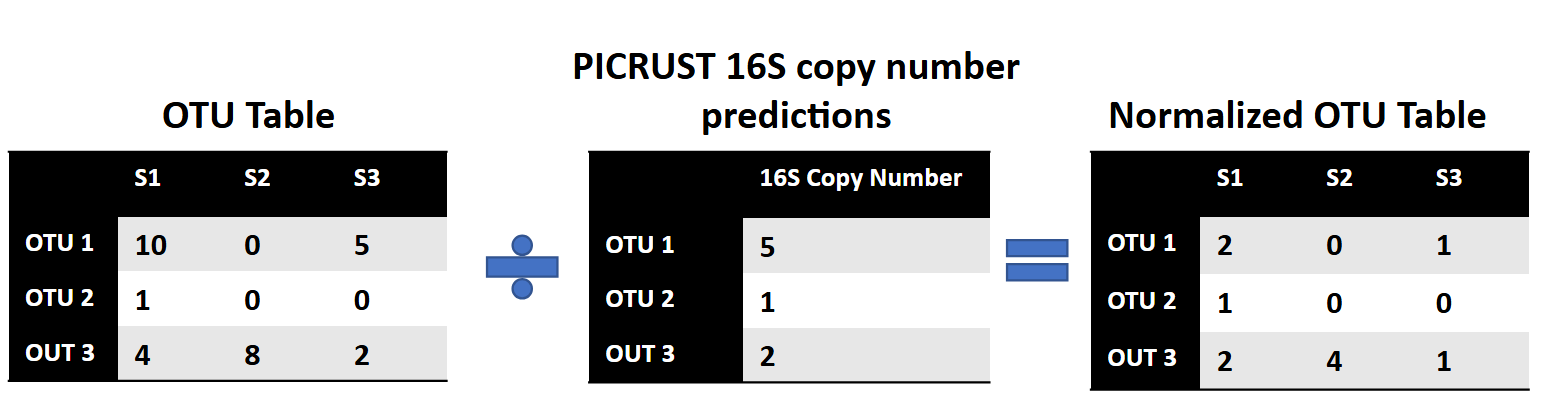
\includegraphics[width = \textwidth]{figs/picrust-normalizacion.png}
\end{figure}

Una vez tenemos la especie normalizada, la multiplicamos por una matriz que contiene las predicciones de contenido génico (obtenidas mediante el proceso de predicción del estado ancestral mencionado anteriormente), obteniendo así la predicción del metagenoma deseado. 

Por ejemplo, si queremos saber cómo de abundante es la familia de genes K0001 en S1, y vemos que S1 tiene especies OTU1, OTU2 y OTU3 con abundancias 2, 1 y 2, y que K0001 está presente en esas especies con abundancias 4, 1 y 2. Por lo tanto, hay 2 bacterias de OTU1, OTU2 y OTU3 con abundancias 2, 1 y 2. Por lo tanto, hay 2 bacterias de OTU1 con 4 copias de K0001 cada una, más 1 OTU2 con 1 copia y 2 de OTU3 con 2 copias cada una, luego: 2*4+1*1+2*2=13 copias del gen en el metagenoma.

\begin{figure}[h]
\centering
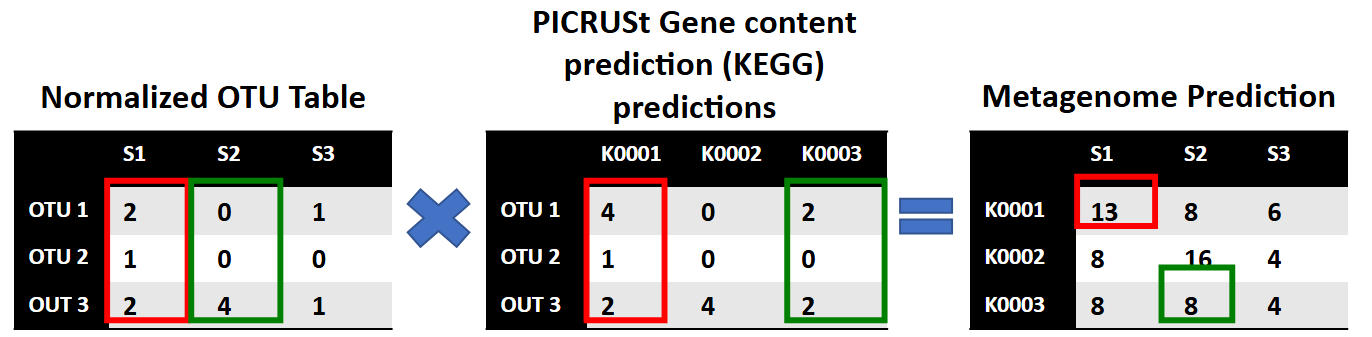
\includegraphics[width = \textwidth]{figs/picrust-prediccion.png}
\end{figure}

Existe una tendencia general a la disminución de la precisión de PICRUSt con el aumento de la distancia media 16S al genoma de referencia más cercano.
Si las especies de nuestra muestra no tienen genomas anotados estrechamente relacionados en la base de datos, PICRUSt no será preciso.
Importante: PICRUST sólo funciona con el protocolo «closed-reference OTU picking». No se permite de novo OUT picking (no tenemos un genoma de referencia para extraer / predecir genes).

Aunque no se puede confiar completamente en los resultados de la predicción metagenómica, es una herramienta muy útil. En este sentido, existen otras herramientas similares, pero PICRUSt es la que mejor funciona, y existe una versión mejorada recientemente (PICRUSt2, que es un poco mejor que PICRUSt).

\subsection{Práctica}
\begin{lstlisting}
conda activate ngs
gdown 1oq3D23KBaJ5UhVh--eVL6fa50oIpGl0m
unzip picrust_example.zip
conda deactivate ngs

conda create -n picrust -c bioconda picrust -y

# Download pre-computed database files
conda activate picrust
download_picrust_files.py
conda deactivate

# conda activate picrust
normalize_by_copy_number.py -i otus.biom -o otus_corrected.biom 

biom convert -i otus.biom -o otus.txt --to-tsv --header-key taxonomy
biom convert -i otus_corrected.biom -o otus_corrected.txt --to-tsv --header-key taxonomy

predict_metagenomes.py -i otus_corrected.biom -o ko_predictions.biom

biom convert -i ko_predictions.biom -o ko_predictions.txt --to-tsv --header-key KEGG_Description   

# sudo apt-get install gawk
# brew install gawk
# Less try to compare functional genes from 2 samples (healthy mouse on column 2 vs sick mouse on column 11)
gawk 'NR>2{if ($2 > 0 && $11 > 0 ) print $1 " #00ff00 W10"}' < ko_predictions.txt > ko.txt
gawk 'NR>2{if ($2 > 0 && $11 == 0 ) print $1 " #ff0000 W10"}' < ko_predictions.txt >> ko.txt
gawk 'NR>2{if ($2 == 0 && $11 > 0 ) print $1 " #0000ff W10"}' < ko_predictions.txt >> ko.txt
\end{lstlisting}

Los resultados se copian en la página de iPATH3 y se pincha en metabolismo (pathway maps > metabolic pathways). Esta página crea un mapa con todos los genes metabólicos presentes en nuestros datos. 

PICRUSt también puede colapsar KOs a KEGG Pathways. Hay que tener en cuenta que una KO puede asignarse a muchas rutas KEGG, por lo que una simple asignación no funcionaría aquí. En su lugar, utilizamos el script de PICRUSt "categorize\_by\_function.py":
\begin{lstlisting}
categorize_by_function.py -i ko_predictions.biom -c KEGG_Pathways -l 3 -o pathway_predictions.biom

biom convert -i pathway_predictions.biom -o pathway_predictions.txt --to-tsv --header-key KEGG_Pathways

python biom_to_stamp.py -m KEGG_Pathways pathway_predictions.biom > pathway_predictions.spf

conda deactivate
conda activate stamp
STAMP
\end{lstlisting}